\begin{figure}[t]
\vspace*{-2ex}
\centering
\begin{subfigure}{.22\textwidth}
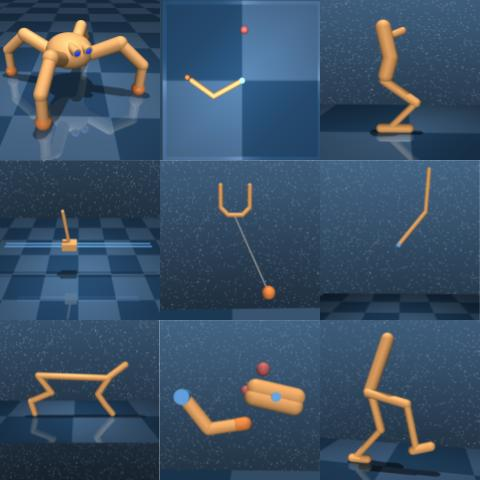
\includegraphics[width=\linewidth]{tasks/dmc}
\caption{Control Suite}
\end{subfigure}\hfill
\begin{subfigure}{.22\textwidth}
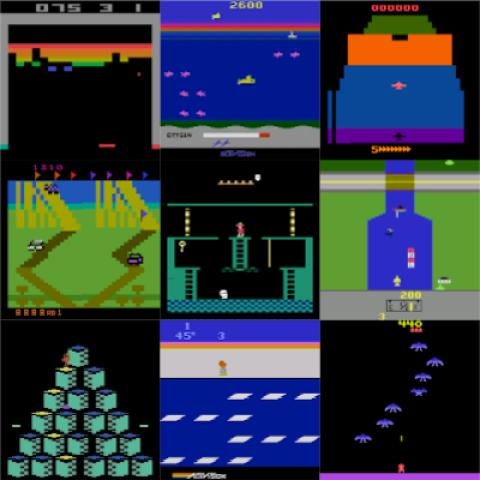
\includegraphics[width=\linewidth]{tasks/atari}
\caption{Atari}
\end{subfigure}\hfill
\begin{subfigure}{.22\textwidth}
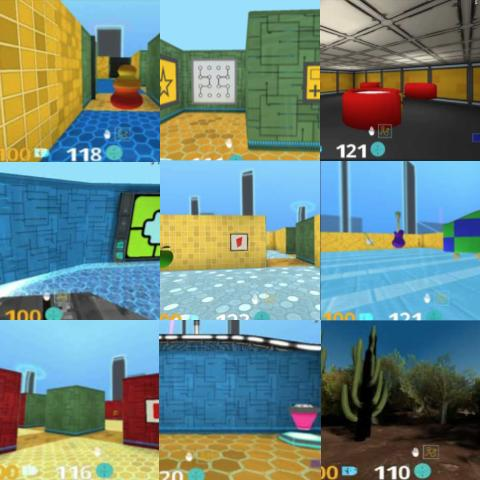
\includegraphics[width=\linewidth]{tasks/dmlab}
\caption{DMLab}
\end{subfigure}\hfill
\begin{subfigure}{.22\textwidth}
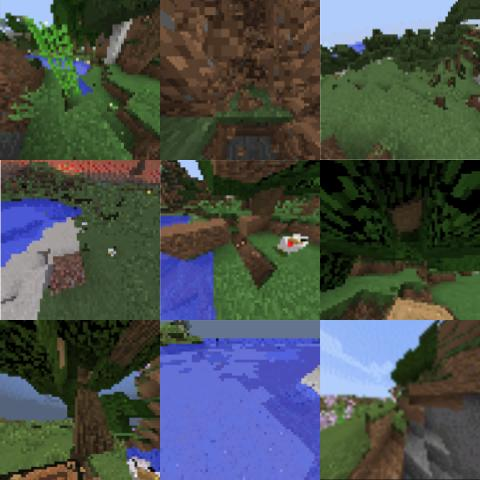
\includegraphics[width=\linewidth]{tasks/minecraft}
\caption{Minecraft}
\end{subfigure}
\caption{Four visual domains considered in this work. DreamerV3 succeeds across these diverse domains, ranging from robot locomotion and manipulation tasks over Atari games with 2D graphics to complex 3D domains such as DMLab and Minecraft that require spatial and temporal reasoning.}
\label{fig:tasks}
\end{figure}
